% =============================================================================
%  SEML Companion Reader — Session 2: ML in Production
%  AIMLCZG546 · BITS Pilani
% =============================================================================
\documentclass[a4paper,11pt]{article}

% ---- Encoding & fonts -------------------------------------------------------
\usepackage[T1]{fontenc}
\usepackage[utf8]{inputenc}
\usepackage{lmodern}
\usepackage{microtype}

% ---- Geometry ---------------------------------------------------------------
\usepackage[a4paper,margin=1in,headheight=15pt,headsep=14pt]{geometry}

% ---- Math -------------------------------------------------------------------
\usepackage{amsmath,amssymb}

% ---- Graphics, tables, colour -----------------------------------------------
\usepackage{graphicx}
\usepackage{booktabs}
\usepackage{adjustbox}
\usepackage[table,svgnames]{xcolor}

% ---- Callout boxes ----------------------------------------------------------
\usepackage[most]{tcolorbox}
\tcbuselibrary{skins,breakable}

% ---- Tikz -------------------------------------------------------------------
\usepackage{tikz}

% ---- Glyphs: pifont only (bbding command names vary across TeX installs) ----
\usepackage{pifont}
\newcommand{\glyphHand}{\ding{43}}
\newcommand{\glyphPencil}{\ding{46}}

% ---- Lists & spacing --------------------------------------------------------
\usepackage{enumitem}
\setlist{leftmargin=1.5em,topsep=4pt,itemsep=3pt}

% ---- Steps list for worked examples (keeps "Step N." inside callout box) ----
\newlist{steps}{enumerate}{1}
\setlist[steps]{label=\textbf{Step \arabic*.},
  leftmargin=4.4em, labelwidth=3.8em, labelsep=0.6em, labelindent=0pt,
  align=left, topsep=5pt, itemsep=6pt}

\usepackage{parskip}

% ---- Headers / footers ------------------------------------------------------
\usepackage{fancyhdr}

% ---- Section styling --------------------------------------------------------
\usepackage{titlesec}

% ---- Links + URL line-breaking ----------------------------------------------
\usepackage[hidelinks]{hyperref}
\usepackage{xurl}
\hypersetup{breaklinks=true}

% =============================================================================
%  COLOURS
% =============================================================================
\definecolor{navy}{HTML}{21355E}
\definecolor{navyrule}{HTML}{21355E}
\definecolor{inktext}{HTML}{1A202C}
\definecolor{mutedtext}{HTML}{6B7280}

\definecolor{intuFrame}{HTML}{2C5AA0}   \definecolor{intuFill}{HTML}{F4F7FC}
\definecolor{everyFrame}{HTML}{8A5A1E}  \definecolor{everyFill}{HTML}{FBF1E3}
\definecolor{workFrame}{HTML}{2E7D52}   \definecolor{workFill}{HTML}{F1F8F3}
\definecolor{watchFrame}{HTML}{B23A48}  \definecolor{watchFill}{HTML}{FBF1F2}
\definecolor{keyFrame}{HTML}{6A4C93}    \definecolor{keyFill}{HTML}{F4F0F9}

\color{inktext}
\hypersetup{linkcolor=navy,urlcolor=navy,citecolor=navy}

% =============================================================================
%  CALLOUT BOXES
% =============================================================================
\tcbset{
  housecallout/.style 2 args={
    enhanced, breakable,
    colback=#2, colframe=#1,
    boxrule=0.6pt, arc=2.4pt, outer arc=2.4pt,
    left=10pt, right=10pt, top=9pt, bottom=9pt,
    before skip=11pt, after skip=11pt,
    fontupper=\normalsize,
    coltitle=white,
    fonttitle=\bfseries\sffamily\small,
    attach boxed title to top left={xshift=6mm,yshift=-3mm},
    boxed title style={
      colback=#1, colframe=#1,
      rounded corners, arc=3pt,
      boxrule=0pt, left=6pt, right=6pt, top=2pt, bottom=2pt
    }
  }
}

\newtcolorbox{intuition}{%
  housecallout={intuFrame}{intuFill},
  title={\raisebox{-0.05ex}{\glyphHand}\,\ The intuition}}

\newtcolorbox{everyday}{%
  housecallout={everyFrame}{everyFill},
  title={\raisebox{-0.05ex}{$\bigstar$}\,\ Everyday picture}}

\newtcolorbox{worked}[1]{%
  housecallout={workFrame}{workFill},
  title={\raisebox{-0.05ex}{\glyphPencil}\,\ Worked example: #1}}

\newtcolorbox{watchout}{%
  housecallout={watchFrame}{watchFill},
  title={\raisebox{-0.05ex}{\ding{55}}\,\ Watch out}}

\newtcolorbox{keytake}{%
  housecallout={keyFrame}{keyFill},
  title={\raisebox{-0.05ex}{\ding{51}}\,\ Key takeaway}}

% =============================================================================
%  TITLE BANNER
% =============================================================================
\providecommand{\addfontfeatureslike}[1]{#1}
\newcommand{\titlebanner}[4]{%
  \begin{tcolorbox}[
    enhanced, breakable=false,
    colback=navy, colframe=navy,
    boxrule=0pt, arc=3pt, outer arc=3pt,
    left=16pt, right=16pt, top=16pt, bottom=16pt,
    before skip=2pt, after skip=14pt,
    width=\linewidth ]
    {\sffamily\footnotesize\bfseries\color{white!85}%
      \MakeUppercase{\addfontfeatureslike{#1}}}\par
    \vspace{6pt}
    {\sffamily\bfseries\fontsize{30}{34}\selectfont\color{white} #2\par}
    \vspace{5pt}
    {\sffamily\large\color{white!88} #3\par}
    \vspace{9pt}
    {\color{white!55}\rule{\linewidth}{0.4pt}}\par
    \vspace{6pt}
    {\sffamily\footnotesize\color{white!82} #4\par}
  \end{tcolorbox}%
}

% =============================================================================
%  \housefig{path}{caption}
% =============================================================================
\newcommand{\housefig}[2]{%
  \begin{figure}[htbp]
    \centering
    \includegraphics[width=\linewidth]{#1}%
    \caption{#2}
  \end{figure}%
}

\newcommand{\vocab}[1]{\textbf{\color{navy}#1}}

% =============================================================================
%  RUNNING HEADER / FOOTER
% =============================================================================
\newcommand{\CourseShort}{SEML Companion}
\newcommand{\SessionNo}{2}
\newcommand{\LectureTitle}{ML in Production}

\pagestyle{fancy}
\fancyhf{}
\fancyhead[L]{\footnotesize\color{mutedtext}\textsf{\CourseShort}}
\fancyhead[R]{\footnotesize\color{mutedtext}\textsf{Session \SessionNo\ \textperiodcentered\ \LectureTitle}}
\fancyfoot[C]{\footnotesize\color{mutedtext}\thepage}
\renewcommand{\headrulewidth}{0.4pt}
\renewcommand{\footrulewidth}{0pt}
\renewcommand{\headrule}{\hbox to\headwidth{\color{navyrule!55}\leaders\hrule height \headrulewidth\hfill}}

% =============================================================================
%  SECTION HEADINGS
% =============================================================================
\titleformat{\section}
  {\sffamily\Large\bfseries\color{navy}}
  {\thesection}{0.8em}{}
  [{\vspace{2pt}\color{navy!70}\titlerule[0.8pt]}]
\titleformat{\subsection}
  {\sffamily\large\bfseries\color{navy!92}}
  {\thesubsection}{0.7em}{}
\titlespacing*{\section}{0pt}{16pt}{8pt}
\titlespacing*{\subsection}{0pt}{12pt}{4pt}

% =============================================================================
\begin{document}
% =============================================================================

\thispagestyle{fancy}

\titlebanner
  {AIMLCZG546 \textperiodcentered\ Session 2 \textperiodcentered\ Companion Reader}
  {ML in Production}
  {From Research Prototype to Production System}
  {Session 2 \textperiodcentered\ Read alongside the lecture slides \textperiodcentered\ Every slide example worked out in full}

% ---- How to use -------------------------------------------------------------
\noindent\textbf{How to use this companion.}
The slides give you the formulas and diagrams. This reader gives you the \emph{why}.
Every concept is expanded in plain English. Every slide example is worked out step by step.
Five colour-coded boxes guide you.
\textcolor{intuFrame}{\textbf{Blue}} = the core idea in one breath.
\textcolor{everyFrame}{\textbf{Amber}} = a real-life analogy before the math.
\textcolor{workFrame}{\textbf{Green}} = a worked example with real numbers.
\textcolor{watchFrame}{\textbf{Red}} = the common mistake to avoid.
\textcolor{keyFrame}{\textbf{Purple}} = the one line to remember.

\medskip

% =============================================================================
\section{What this session covers}
% =============================================================================

This session answers one big question: what happens to a machine learning model after
the research phase ends?

Here are the five topics we cover, in order:

\begin{enumerate}
  \item \textbf{The production gap} --- why a good model is only the start.
  \item \textbf{ML model vs ML system} --- two very different ways to think about your work.
  \item \textbf{ML and non-ML components} --- how ML fits into the larger software picture.
  \item \textbf{AI paradigms} --- predictive, generative, and agentic AI compared.
  \item \textbf{Case studies} --- Apollo (Baidu) and Microsoft show these ideas in real systems.
\end{enumerate}

% =============================================================================
\section{The Production Gap: Sidney's Startup}
% =============================================================================

Here is a story that plays out over and over in industry.
A researcher builds a great model in a notebook.
The test-set accuracy looks strong.
Everyone is excited.
Then they try to deploy it to real users --- and that is where the real work begins.

\begin{everyday}
Think of a chef who perfects a recipe at home.
It works beautifully for six guests.
Then a restaurant chain wants to serve it to 10{,}000 people per day.
The recipe is only a tiny part of the problem.
The real challenges are sourcing ingredients, training staff, quality control, and managing costs.
Moving from \emph{recipe} to \emph{restaurant} takes far more engineering than cooking the dish.
\end{everyday}

\begin{intuition}
A \vocab{production gap} is the gap between a working research model and a working production system.
The model is just the starting point.
The system around it takes as much work as the model itself.
That system includes data pipelines, serving infrastructure, monitoring, teams, and cost control.
\end{intuition}

In the slide's case study, \vocab{Sidney} builds a speech recognition model.
In the lab it hits 94\,\% accuracy.
In production he runs into seven problems:

\begin{itemize}
  \item \textbf{Noisy data} --- real call audio has background noise and accents not in the training set.
  \item \textbf{Latency} --- the model takes 3 seconds per clip; the product needs under 0.5 seconds.
  \item \textbf{Cost} --- running the model 24\,/\,7 at scale costs 40$\times$ the research estimate.
  \item \textbf{Fragile pipelines} --- the preprocessing script breaks when the call centre upgrades its format.
  \item \textbf{Team gaps} --- ML researchers and software engineers use different tools and vocabulary.
  \item \textbf{Monitoring} --- accuracy drifts for three weeks before anyone notices.
  \item \textbf{Fairness} --- the model is 15\,\% worse on non-native English speakers.
\end{itemize}

\begin{worked}{diagnosing Sidney's 3-second latency}
Sidney's model takes 3 seconds per audio clip. The product requires 0.5 seconds. Let us trace the bottleneck.
\begin{steps}
  \item \textbf{Measure each stage.} Total pipeline time: 3.0 s.
        Preprocessing (resampling, noise filter): 1.8 s.
        Model inference: 0.9 s.
        Postprocessing (text formatting): 0.3 s.
  \item \textbf{Find the biggest cost.} Preprocessing takes 1.8 s --- 60\,\% of the total.
  \item \textbf{Optimise the top item.} Replace the pure-Python noise filter with a compiled C library.
        New preprocessing time: 0.2 s.
  \item \textbf{Re-measure.} New total: $0.2 + 0.9 + 0.3 = 1.4$ s. Still over budget.
  \item \textbf{Optimise inference.} Quantise the model from 32-bit to 8-bit weights.
        New inference time: 0.25 s.
  \item \textbf{Final total.} $0.2 + 0.25 + 0.3 = \mathbf{0.75}$ s. Within budget.
\end{steps}
The bottleneck was \emph{not} the model --- it was the preprocessing step.
A system-centric view found the fix faster.
\end{worked}

\begin{watchout}
Do not assume the model is the bottleneck.
In production systems, data pipelines and infrastructure are often the slow parts.
Profile first, then optimise.
\end{watchout}

\begin{keytake}
Moving from research prototype to production system needs as much engineering as building the model --- often more.
Profile the whole system before you tune the model.
\end{keytake}

\housefig{figures/fig_production_gap.png}{Seven production challenges that Sidney's startup faces.
Latency and cloud cost are the most severe.
Each bar is one challenge that the model alone cannot fix.}

\noindent\textbf{Where this shows up in ML.}
Every deployed ML product --- a recommendation engine, a fraud detector, a language model in a product --- faces this gap.
\vocab{MLOps} (ML Operations) is the discipline that bridges it.
It covers automated pipelines, model registries, monitoring dashboards, and continuous retraining.

% =============================================================================
\section{ML Model vs ML System}
% =============================================================================

There are two very different ways to think about an ML project.

\begin{intuition}
An \vocab{ML model} is the trained function that maps inputs to outputs.
An \vocab{ML system} is the entire product.
It includes data pipelines, the model, serving infrastructure, monitoring, feedback loops, and the team that runs all of it.
The model is one component of the system.
\end{intuition}

\begin{everyday}
An ML model is like the engine in a car.
A better engine helps.
But the car's usefulness also depends on the chassis, the steering, the fuel system, and the dashboard.
Tuning only the engine while ignoring everything else is \emph{model-centric} thinking.
\end{everyday}

\subsection{Model-Centric View}

A \vocab{model-centric} team asks: ``How do we make the model more accurate?''
They tune hyperparameters, try new architectures, and add labelled data.
Progress stops when the model tops out.

\subsection{System-Centric View}

A \vocab{system-centric} team asks: ``How do we make the whole system better for users?''
The model is one part of a larger system.
Gains can come from cleaner data, faster serving, better monitoring, or a better user interface --- not just the model.

\subsection{The Iceberg of Hidden Technical Debt}

Sculley et al.\ (2015) studied ML systems at Google.
They found that the ML model code is only a small fraction of the total codebase.
The rest is infrastructure.

\begin{center}
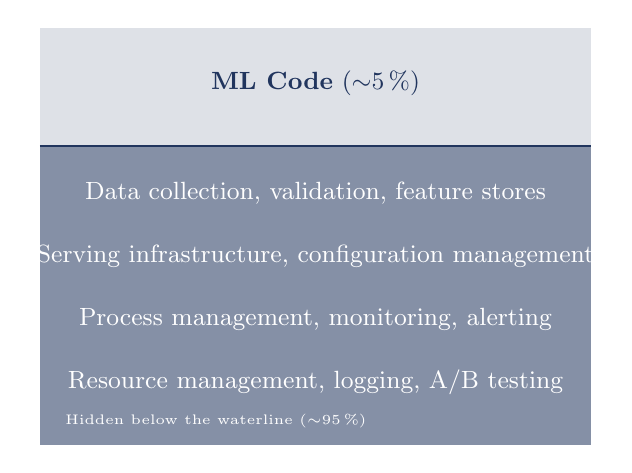
\begin{tikzpicture}[font=\small]
  \fill[navy!15] (-3.5,-0.2) -- (3.5,-0.2) -- (3.5,1.3) -- (-3.5,1.3) -- cycle;
  \fill[navy!55] (-3.5,-4.0) -- (3.5,-4.0) -- (3.5,-0.2) -- (-3.5,-0.2) -- cycle;
  \draw[thick,navy] (-3.5,-0.2) -- (3.5,-0.2);
  \node[align=center,navy] at (0,0.6) {\textbf{ML Code} ($\sim$5\,\%)};
  \node[align=center,white,font=\small] at (0,-0.8) {Data collection, validation, feature stores};
  \node[align=center,white,font=\small] at (0,-1.6) {Serving infrastructure, configuration management};
  \node[align=center,white,font=\small] at (0,-2.4) {Process management, monitoring, alerting};
  \node[align=center,white,font=\small] at (0,-3.2) {Resource management, logging, A/B testing};
  \node[right,white,font=\tiny] at (-3.3,-3.7) {Hidden below the waterline ($\sim$95\,\%)};
\end{tikzpicture}
\end{center}

\housefig{figures/fig_ml_fraction.png}{ML model code is about 5\,\% of a production system.
The other 95\,\% is data work, infrastructure, monitoring, and configuration.
Focus on the whole iceberg, not just the tip.}

\begin{watchout}
Optimising the ML model while ignoring the infrastructure is like polishing an engine while the fuel tank leaks.
The fuel tank will fail first.
\end{watchout}

\begin{worked}{model-centric vs system-centric fraud detection}
A bank's fraud model has 88\,\% precision: 12\,\% of blocked transactions are legitimate.
Two teams try to fix it.
\begin{steps}
  \item \textbf{Model-centric team.} Collect more labelled fraud examples.
        Retrain with XGBoost. New precision: 90\,\%. Time: 3 weeks.
  \item \textbf{System-centric team.} Study why false positives occur.
        Discovery: the feature pipeline uses yesterday's exchange rates for international payments.
        Fix the pipeline (a two-line code change).
        New precision: 93\,\%. Time: 2 days.
  \item \textbf{Compare.} The system-centric team got a larger gain in less time.
        They found the bug by looking \emph{beyond} the model.
\end{steps}
The system-centric view wins here because the root cause was a data pipeline bug, not a model weakness.
\end{worked}

\noindent\textbf{Where this shows up in ML.}
Industry data shows that in most ML projects, 80\,\% of the time goes to data work (collection, cleaning, labelling).
Only 20\,\% goes to model building.
This is the \vocab{80/20 rule of ML engineering}.

\begin{keytake}
The ML model is a small part of the ML system.
System-centric thinking --- looking at data, infrastructure, and monitoring --- usually finds bigger wins faster.
\end{keytake}

% =============================================================================
\section{ML and Non-ML Components in a System}
% =============================================================================

Every production ML product is a mix of ML code and traditional software.
The ML component may be the core of the product or just one supporting feature.

\begin{intuition}
ML is a \emph{component}, not a product.
A transcription service uses ML as its core value.
A tax software product uses ML as one feature (audit risk flagging) alongside many non-ML components.
The ratio of ML to non-ML code shapes the engineering challenges.
\end{intuition}

\begin{everyday}
Think of a car assembly line.
The engine (ML model) is important.
But the line also needs conveyor belts, robotic arms, quality sensors, and human inspectors.
The non-ML parts must be designed to work reliably with the ML part.
\end{everyday}

\noindent Here is how ML fits in three real products:

\begin{center}
\begin{adjustbox}{max width=\linewidth}
\begin{tabular}{lll}
\toprule
\textbf{Product} & \textbf{ML role} & \textbf{Non-ML components} \\
\midrule
Speech transcription & Core (the product is the ML output) & Audio codec, API gateway, billing \\
Tax audit risk tool & Auxiliary (flags for human review) & Form parser, rule engine, tax database \\
E-commerce recommendations & Core (drives revenue) & Product catalogue, cart, payment system \\
\bottomrule
\end{tabular}
\end{adjustbox}
\end{center}

\noindent\vocab{Systems thinking} means you must design every non-ML component around the ML component's failure modes.
When the model makes a mistake, who sees it? What happens next? How do you recover?
These are software engineering questions, not ML questions.

\begin{worked}{what happens when the speech model fails}
The transcription service misidentifies a medical term (``hypertension'' as ``high tension'').
\begin{steps}
  \item \textbf{Detection.} The monitoring system flags a spike in user corrections.
  \item \textbf{Diagnosis.} Log analysis shows the error rate is higher for audio with background noise above 40\,dB.
  \item \textbf{Fix options.} Option A: retrain the model on noisy-audio examples (weeks).
        Option B: add a noise-detection pre-filter that routes noisy clips to a different model (days).
  \item \textbf{Rollback.} While the fix is prepared, the system routes flagged clips to human review.
        This is a non-ML fallback --- a software engineering design decision made before the model was deployed.
\end{steps}
The non-ML fallback (human review routing) kept the product usable while the ML fix was built.
This is why you design the full system, not just the model.
\end{worked}

\begin{watchout}
A product that relies 100\,\% on the ML model with no non-ML fallback will fail visibly when the model makes a mistake.
Always design for graceful degradation.
\end{watchout}

\noindent\textbf{Where this shows up in ML.}
The field of \vocab{responsible AI} requires non-ML checks: bias audits, fairness dashboards, human-in-the-loop review, and audit logs.
These are all non-ML components that wrap the ML model.

\begin{keytake}
ML is one component in a larger system.
Design the whole system --- including how the non-ML parts handle model errors --- before you deploy.
\end{keytake}

\housefig{figures/fig_ml_component_share.png}{How much of each product is ML.
Speech transcription is almost entirely ML.
Tax audit risk flagging is mostly non-ML.
E-commerce recommendations are mostly ML.
The mix changes the engineering approach.}

% =============================================================================
\section{The ML Pipeline: From Data to Deployment}
% =============================================================================

A \vocab{machine learning pipeline} is the sequence of steps that turns raw data into a running model.
In research, the pipeline is mostly a one-time process.
In production, the pipeline is a cycle that never stops.

\housefig{figures/fig_pipeline.png}{The 7-stage ML pipeline.
Stages 1--4 are all data work.
In production, the pipeline is a loop: new data feeds back into training, and the deployed model feeds back into monitoring.}

\begin{intuition}
Think of the pipeline as a factory assembly line.
Raw material (data) comes in at one end.
A finished product (deployed model) comes out the other end.
Each station on the line transforms the material.
If any station breaks, the factory stops.
\end{intuition}

The key stages are:

\begin{enumerate}
  \item \textbf{Data collection} --- gather labelled examples from real-world sources.
  \item \textbf{Data cleaning} --- remove noise, fix errors, handle missing values.
  \item \textbf{Feature engineering} --- turn raw data into numbers the model can learn from.
  \item \textbf{Model training} --- fit the model to the training set.
  \item \textbf{Model evaluation} --- check performance on a held-out set.
  \item \textbf{Deployment} --- serve the model to real users via an API.
  \item \textbf{Monitoring} --- watch for data drift, accuracy drops, and cost spikes.
\end{enumerate}

In production, Stage 7 loops back to Stage 1.
New production data is collected, cleaned, and used to retrain the model.
This cycle is called \vocab{continuous training}.

\begin{watchout}
A static pipeline (train once, deploy forever) will degrade over time.
Real-world data changes: new slang, new products, new user behaviours.
A model trained last year on last year's data will make mistakes on this year's inputs.
\end{watchout}

\noindent\textbf{Where this shows up in ML.}
\vocab{MLOps} tools (Kubeflow, MLflow, Airflow, Vertex AI Pipelines) automate this cycle.
They version every dataset, every model, and every experiment.
They trigger retraining when monitoring detects drift.

\begin{keytake}
The ML pipeline is a loop, not a line.
Monitoring and retraining are as important as training itself.
\end{keytake}

% =============================================================================
\section{AI Paradigms: Predictive, Generative, and Agentic}
% =============================================================================

Modern AI systems fall into three paradigms.
Each has different capabilities and different engineering requirements.

\begin{intuition}
\textbf{Predictive AI} answers a question: ``Will this customer churn?'' \\
\textbf{Generative AI} creates something new: ``Write me an email.'' \\
\textbf{Agentic AI} achieves a goal: ``Book me a flight, write the agenda, and send the invite.''
Each paradigm is more powerful and more complex than the last.
\end{intuition}

\subsection{Predictive AI}

\vocab{Predictive AI} uses past data to forecast future outcomes.
You train a model on historical examples.
The model answers a fixed question: a label, a number, or a probability.
Output: one answer per input.

Examples: spam filter, fraud detector, churn predictor, demand forecast.

\subsection{Generative AI}

\vocab{Generative AI} creates new content from patterns it learned.
A \vocab{foundation model} (a large model pre-trained on huge data) is given a natural-language instruction.
It produces a digital artefact: text, code, an image, or a video.

The slide defines it precisely:
``A system based on a foundation model that generates digital artefacts based on natural user instructions.''
The key word is \emph{generates} --- the output is new, not just a category.

\subsection{Agentic AI}

\vocab{Agentic AI} acts on its own to reach a goal.
It can reason: plan multi-step actions.
It can use tools: call APIs, search the web, run code.
It can reflect: check its own output and try again.

The slide gives three definitions that all point to the same idea:

\begin{center}
\begin{adjustbox}{max width=\linewidth}
\begin{tabular}{lp{9cm}}
\toprule
\textbf{Source} & \textbf{Definition} \\
\midrule
Nvidia & Uses reasoning and planning to solve complex, multi-step problems. \\
OpenAI & Pursues complex goals with limited direct supervision. \\
Schneider (2025) & A foundation-model system that plans, reflects, and uses tools. \\
\bottomrule
\end{tabular}
\end{adjustbox}
\end{center}

The key formula from the slide:
\[
\text{Agentic AI} = \text{Generative AI} + \text{Reasoning} + \text{Tools} + \text{Feedback Loops}
\]

\begin{everyday}
Predictive AI is a weather-forecast app: you ask one question, it gives one answer.
Generative AI is a ghostwriter: you say ``draft the email'' and it writes the email.
Agentic AI is a personal assistant.
You say ``handle the trip.''
It books the flight, writes the agenda, sends the invite, and revises the plan when the venue changes.
\end{everyday}

\housefig{figures/fig_ai_paradigms.png}{The three AI paradigm types ranked by autonomy.
Predictive AI answers one question. Generative AI creates content.
Agentic AI pursues a goal through a sequence of actions.
Each step up adds more autonomy and more engineering complexity.}

\begin{worked}{classifying three AI products}
Three products are described. Classify each as predictive, generative, or agentic.
\begin{steps}
  \item \textbf{Product A:} ``Given a customer's purchase history, predict whether they will buy again this month.''
        Output: a probability (one number). The model answers a fixed question.
        \textbf{Classification: Predictive AI.}
  \item \textbf{Product B:} ``Given a product name and description, write three marketing headlines.''
        Output: new text. The system creates content.
        \textbf{Classification: Generative AI.}
  \item \textbf{Product C:} ``Find the cheapest flight to Singapore next week. Book it.
        Apply my loyalty points and confirm the booking.''
        The system searches databases, compares prices, and takes action.
        Output: a completed multi-step action. The system plans and acts.
        \textbf{Classification: Agentic AI.}
\end{steps}
The key test: does it answer one question (predictive), create content (generative), or plan and act on its own (agentic)?
\end{worked}

\begin{watchout}
Agentic AI is not just a smarter chatbot.
It can take real-world actions: send emails, make purchases, delete files.
This changes the SE challenges.
You must design safety guardrails, rollback mechanisms, and human checkpoints.
\end{watchout}

\noindent\textbf{Where this shows up in ML.}
Most production ML products today are predictive.
Generative AI products are growing fast.
Agentic AI is the next frontier: it requires new SE practices (agent orchestration, tool safety, audit logs, and human oversight).

\begin{keytake}
Predictive AI answers one question. Generative AI creates content. Agentic AI achieves a goal.
Each step up the ladder adds more power and more engineering complexity.
\end{keytake}

% =============================================================================
\section{Case Study: Apollo Autonomous Driving (Baidu)}
% =============================================================================

Baidu's Apollo platform is one of the most complex ML systems ever built.
It shows what ``ML system'' means at industrial scale.

\begin{intuition}
Apollo is a self-driving car platform.
It uses \textbf{28 ML models} working together in real time.
No single model does all the work.
Each model handles one task and passes its output to the next model.
The whole pipeline runs 30 times per second.
\end{intuition}

\begin{everyday}
Think of a surgery team.
The anaesthetist, surgeon, and scrub nurse each do one specialised job.
Their outputs feed into each other.
If one person makes an error, it affects everyone downstream.
Apollo's 28 models work the same way.
\end{everyday}

\noindent Apollo's models cover three areas:

\begin{itemize}
  \item \textbf{Perception} --- cameras and LiDAR see lanes, vehicles, pedestrians, and signs.
  \item \textbf{Detection and classification} --- models label each object and predict its type.
  \item \textbf{Trajectory prediction} --- models forecast where each object will be in the next 3--5 seconds.
\end{itemize}

\housefig{figures/fig_apollo_pipeline.png}{Apollo's 7-stage perception pipeline.
Each box is a model or a processing step.
The output of one box is the input to the next.
A miss at any stage (for example, failing to detect a pedestrian) causes errors in all later stages.}

\begin{worked}{tracing a cascading failure in Apollo}
A camera frame arrives. The Object Detection model misses one pedestrian (a false negative).
\begin{steps}
  \item \textbf{Detection stage.} Object Detection outputs 13 bounding boxes (missed the pedestrian).
  \item \textbf{Classification stage.} The 13 boxes are classified. The pedestrian is not in any box.
  \item \textbf{Sensor fusion.} LiDAR points from the pedestrian are present, but the fusion model
        has no detection to attach them to. The pedestrian is not in the 3D map.
  \item \textbf{Trajectory prediction.} No pedestrian in the 3D map. No trajectory is predicted.
  \item \textbf{Motion planning.} The planner sees no obstacle. It does not slow down or steer around the person.
  \item \textbf{Outcome.} The vehicle continues at speed. This is a safety-critical failure caused by one false negative in Step 1.
\end{steps}
This is a \vocab{cascading failure}: one error in an early model propagates through all later models.
It shows why SE practices (redundancy, sensor fusion, safety stops) are as important as model accuracy.
\end{worked}

\noindent\textbf{SE challenges in Apollo:}
\begin{itemize}
  \item \textbf{High complexity.} 28 interacting models must all be tested together.
  \item \textbf{Low test coverage.} Probabilistic models are hard to unit-test.
  \item \textbf{Model maintenance.} Each of the 28 models must be versioned and retrained separately.
  \item \textbf{Safety requirements.} A wrong prediction can harm a person.
\end{itemize}

\noindent\textbf{Where this shows up in ML.}
Apollo illustrates all four SE challenges from the lecture.
Multi-source data fusion, model interaction design, and safety-critical testing are active research areas in ML systems engineering.

\begin{keytake}
A real ML system is not one model.
It is many models working together.
A single model's mistake can cascade through the whole system.
SE practices --- redundancy, fallbacks, and testing --- protect against this.
\end{keytake}

% =============================================================================
\section{Case Study: Microsoft's 9-Stage ML Workflow}
% =============================================================================

Microsoft studied how software teams build ML products.
They found a consistent 9-stage workflow and key lessons about how ML development differs from traditional software.

\begin{intuition}
Traditional software development has a plan: gather requirements, design, code, test, deploy.
ML development has a loop: gather requirements, get data, clean data, label data, engineer features, train, evaluate, deploy, monitor.
Then the loop starts again.
The big difference is that \emph{data} is the central engineering activity, not code.
\end{intuition}

\housefig{figures/fig_ms_workflow.png}{Microsoft's 9-stage ML workflow.
Stages 1--5 (left half) are all about data.
Only Stage 6 (model training) and Stage 7 (evaluation) are traditional ML.
Stages 8 and 9 (deployment and monitoring) connect the model to production.}

\begin{center}
\begin{adjustbox}{max width=\linewidth}
\begin{tabular}{rp{3.8cm}p{6cm}}
\toprule
\textbf{Stage} & \textbf{Name} & \textbf{Key question} \\
\midrule
1 & Model Requirements & What problem are we solving? \\
2 & Data Collection & Where does the data come from? \\
3 & Data Cleaning & Is the data accurate and complete? \\
4 & Data Labelling & Do we have ground truth? Who labels it? \\
5 & Feature Engineering & What signals will help the model? \\
6 & Model Training & What algorithm and hyperparameters? \\
7 & Model Evaluation & Does it meet the performance target? \\
8 & Deployment & How is the model served at scale? \\
9 & Monitoring & Is the model still working well? \\
\bottomrule
\end{tabular}
\end{adjustbox}
\end{center}

\begin{everyday}
Think of building a house.
Stage 1 is the blueprint.
Stages 2--5 are all the groundwork: digging foundations, laying pipes, pouring concrete.
Stage 6 is framing the walls.
Stage 7 is the inspection.
Stages 8--9 are moving in and maintaining the house.
Most people see only the framing (Stage 6). The groundwork (Stages 2--5) is what takes the time.
\end{everyday}

\begin{worked}{why data labelling slows down real teams (Stage 4)}
A team wants to train a model to detect defects in factory photos.
\begin{steps}
  \item \textbf{Collect images.} The factory cameras produce 10{,}000 photos per day.
        Storing one week of data: 70{,}000 images.
  \item \textbf{Sample for labelling.} The team needs 5{,}000 labelled images to train.
        They randomly sample 5{,}000 from the 70{,}000.
  \item \textbf{Label the images.} Each image needs a human expert to mark defect regions.
        Time per image: 2 minutes. Total: $5{,}000 \times 2 = 10{,}000$ minutes $= 167$ hours.
        With two labellers working 8 hours per day: $167 \div 16 \approx \mathbf{10}$ \textbf{working days}.
  \item \textbf{Quality check.} A second labeller re-checks 10\,\% of labels.
        Disagreement rate: 8\,\%. Those 400 images need a third labeller to adjudicate.
  \item \textbf{Total cost.} Two full-time labellers for two weeks, plus domain-expert time for adjudication.
        This is \emph{before} any model training begins.
\end{steps}
This is why Microsoft found that data work (Stages 2--4) dominates ML project timelines.
\end{worked}

\noindent Key findings from Microsoft's research:

\begin{itemize}
  \item \textbf{Data is the core.} Teams spend more time on Stages 2--5 than on Stages 6--7.
  \item \textbf{Iteration is the rule.} Teams run dozens of experiments before picking a model.
  \item \textbf{Cross-functional teams are needed.} ML engineers, data engineers, domain experts, and product managers must work together from Stage 1.
  \item \textbf{Versioning is not optional.} Both models and datasets must be versioned.
\end{itemize}

\begin{watchout}
``We'll fix the data later'' is one of the most expensive sentences in ML.
Data quality problems found after model training require going back to Stage 3 or 4.
That means re-cleaning, re-labelling, and retraining --- weeks of work lost.
Fix data quality before you train.
\end{watchout}

\noindent\textbf{Where this shows up in ML.}
\vocab{Data-centric AI} (Andrew Ng's term) is the practice of treating data quality as the primary engineering activity.
Tools like \vocab{Label Studio}, \vocab{Scale AI}, and \vocab{Snorkel} automate parts of the labelling and cleaning stages.

\begin{keytake}
In the Microsoft workflow, model training is Stage 6 out of 9.
Four data stages come before it.
``Data first, model second'' is the industrial reality.
\end{keytake}

% =============================================================================
\section*{Glossary \& Symbols}
\addcontentsline{toc}{section}{Glossary \& Symbols}
% =============================================================================

\noindent\textbf{Key terms.}
\begin{description}[leftmargin=8.5em,style=nextline,font=\normalfont\bfseries\color{navy}]
  \item[production gap] the gap between a working research model and a working production system.
  \item[ML system] the full product: data pipelines, model, serving, monitoring, and team.
  \item[ML model] the trained function that maps inputs to outputs; one part of the ML system.
  \item[model-centric] a mindset that focuses only on improving the model's accuracy.
  \item[system-centric] a mindset that looks at the whole system to find the best improvement.
  \item[ML pipeline] the sequence of steps from raw data to a deployed model.
  \item[continuous training] automatically retraining the model as new production data arrives.
  \item[MLOps] practices and tools for running ML systems reliably in production.
  \item[predictive AI] AI that uses past data to answer a fixed question (label, number, probability).
  \item[generative AI] AI that creates new content (text, image, code) from a natural instruction.
  \item[agentic AI] AI that plans and takes sequences of real-world actions to achieve a goal.
  \item[foundation model] a large model pre-trained on huge data; fine-tuned for specific tasks.
  \item[cascading failure] one model's error propagates through all downstream models.
  \item[data-centric AI] the practice of treating data quality as the primary engineering activity.
\end{description}

\medskip
\noindent\textbf{Symbols at a glance.}
\begin{center}\small
\begin{tabular}{@{}ll@{}}
\toprule
\textbf{Symbol / term} & \textbf{Meaning} \\
\midrule
$\sim$5\,\% ML code & the fraction of a production system that is model code \\
$\sim$95\,\% hidden & the fraction that is infrastructure (Sculley et al., 2015) \\
28 models & number of ML models in Apollo (Baidu's autonomous driving system) \\
9 stages & Microsoft's ML workflow: 5 data stages + training + eval + deploy + monitor \\
Stage 4 & data labelling: usually the most time-consuming stage \\
\bottomrule
\end{tabular}
\end{center}

\end{document}
